\subsection{Exobolygók detektálása}

\begin{frame}{}
    \centering
    \Huge{Exobolygók detektálása a Kepler-80 és Kepler-90 rendszerekben}\\
    \vspace*{1cm}
    \large{Shallue, Christopher J.; Vanderburg, Andrew \\ \href{https://iopscience.iop.org/article/10.3847/1538-3881/aa9e09/pdf}{Identifying Exoplanets with Deep Learning: A Five-planet Resonant Chain around Kepler-80 and an Eighth Planet around Kepler-90}. \\ The Astronomical Journal, Volume 155, Issue 2, article id. 94, 21 pp. (2018)}
\end{frame}

\begin{frame}
	\frametitle{Kepler}
	\begin{columns}
		\begin{column}{0.5\textwidth}
			\begin{itemize}
				\item NASA Discovery Program
				\item 2009.03.07. Cape Canaveral
				\item First light: 2009.04.08.
				\item 95 cm Schidt távcső
				\item 42 db 2200x1024 CCD
			\end{itemize}
		\end{column}
		\begin{column}{0.5\textwidth}
			\hspace*{0.7cm}
			\vspace{-3cm}
			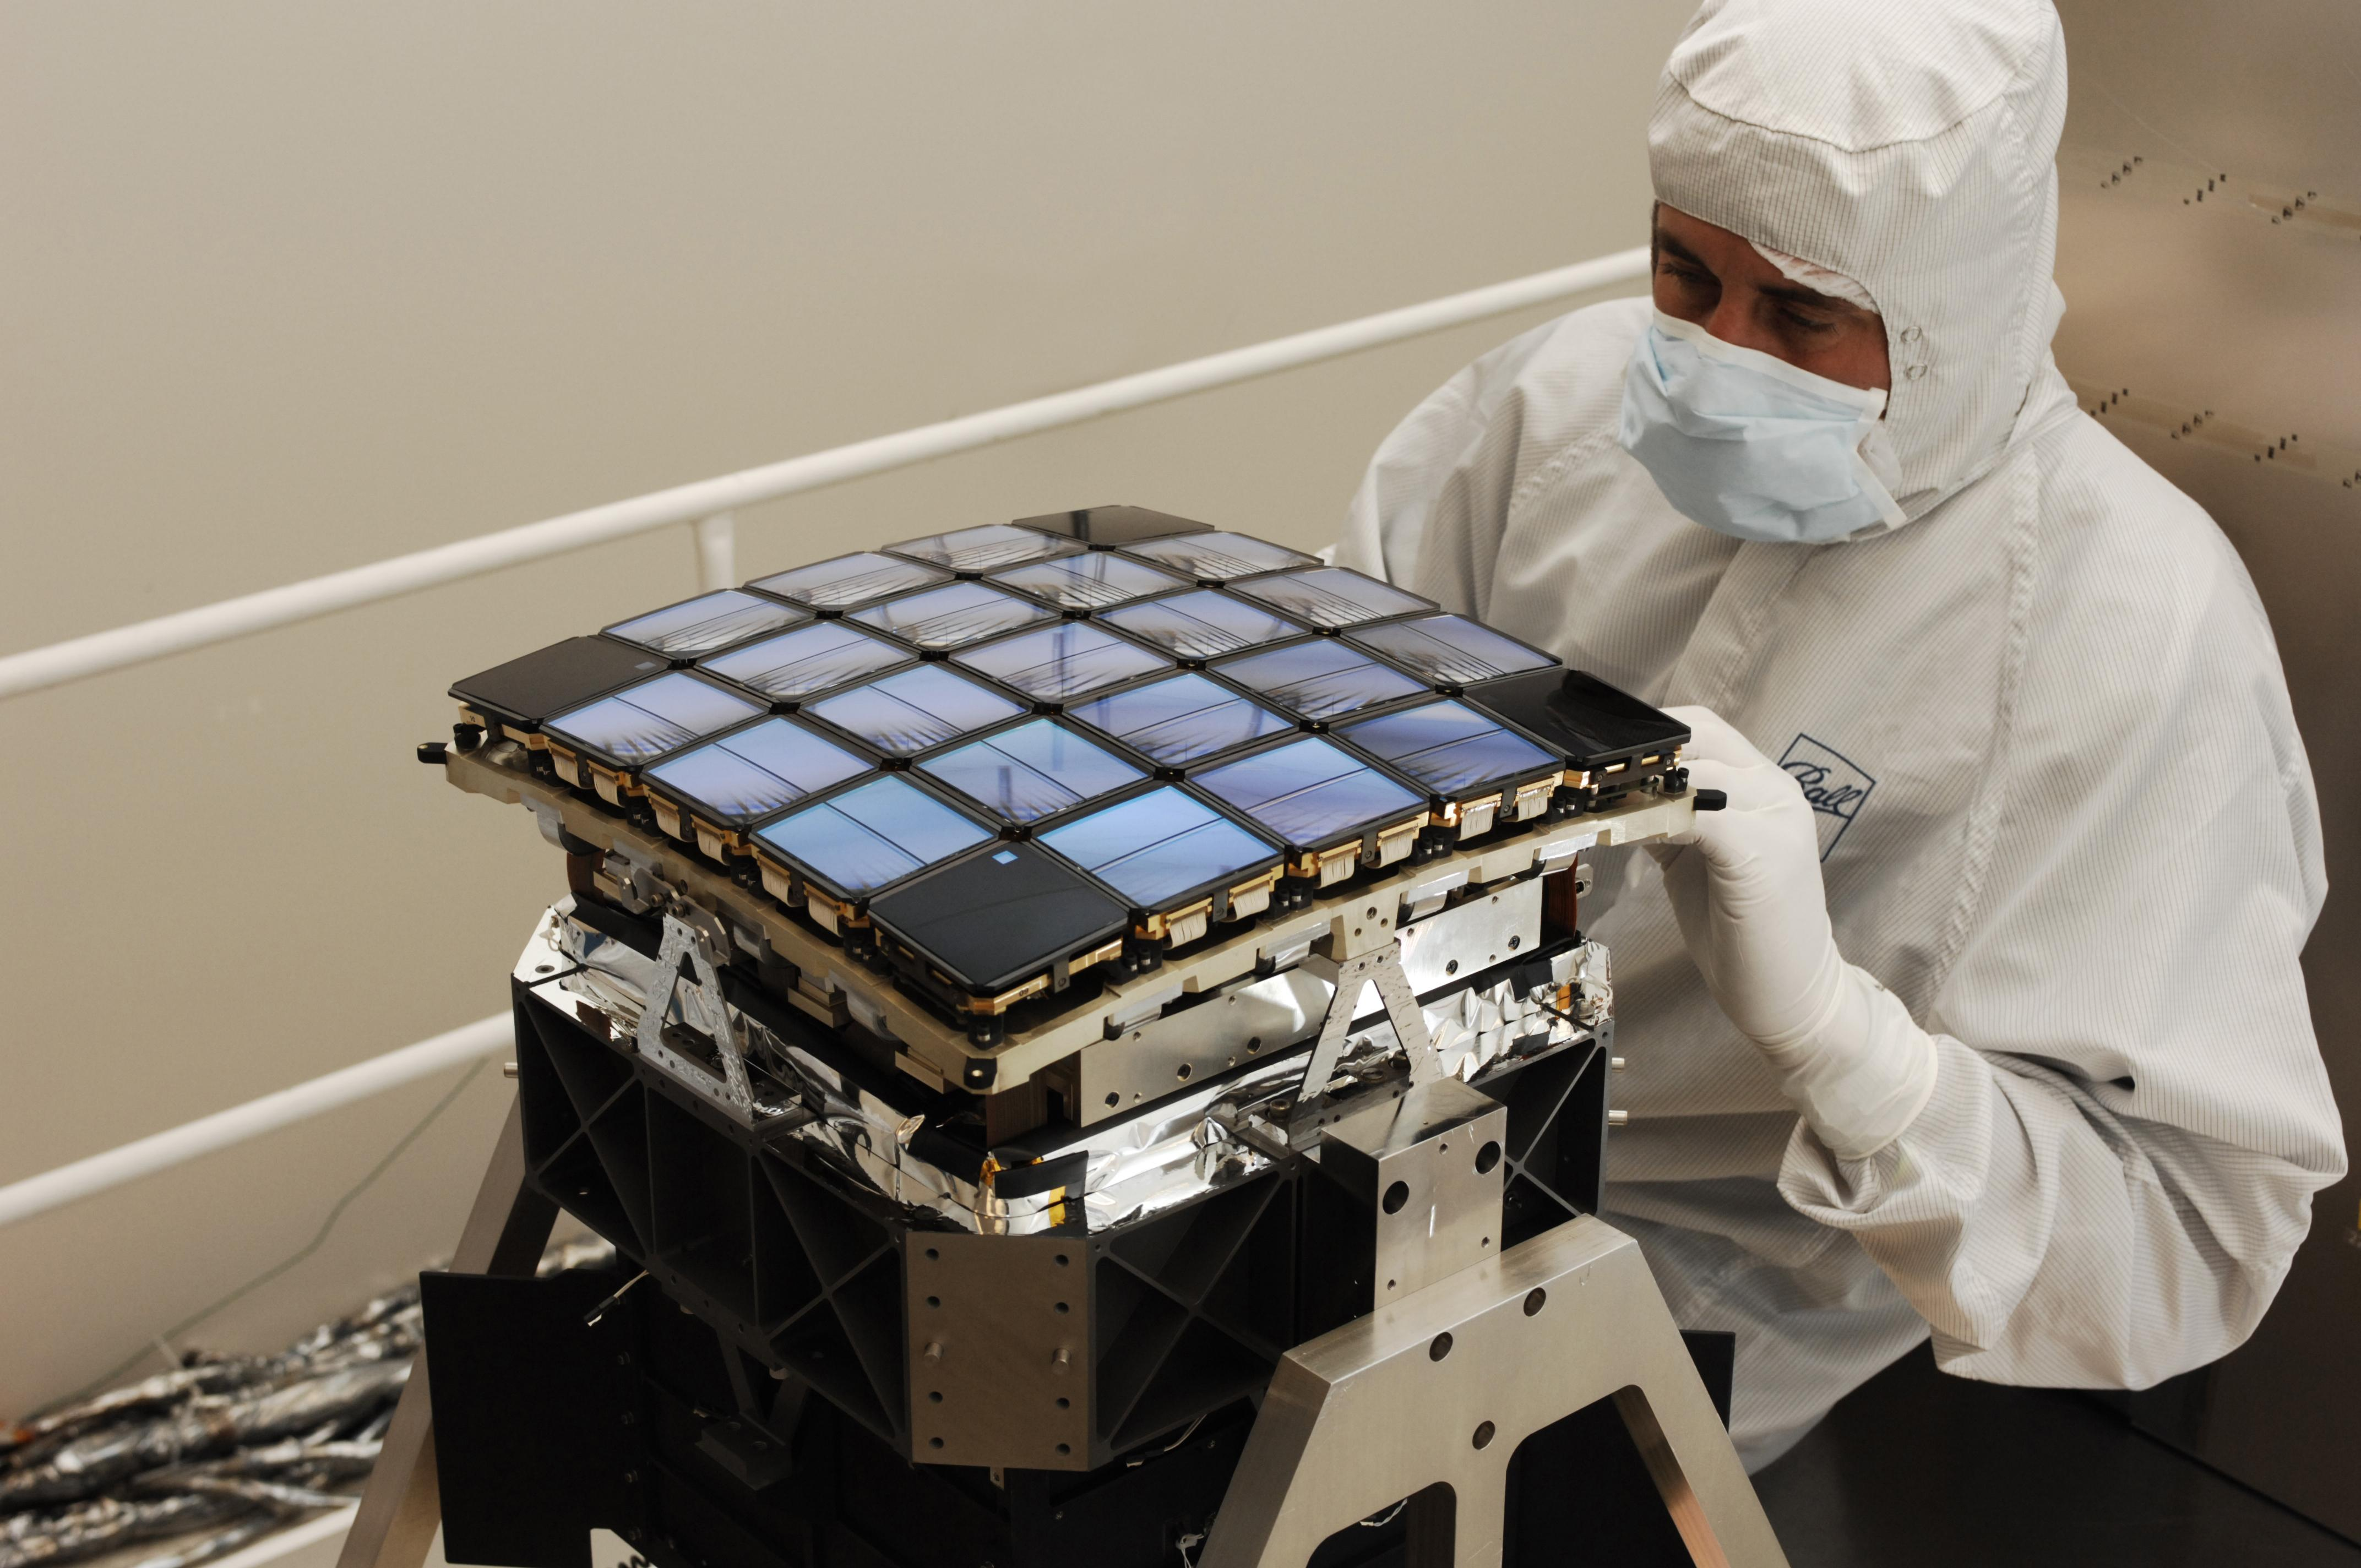
\includegraphics[width=0.9\textwidth]{figures/kepler_eye.jpg}
		\end{column}
		\begin{column}{0.5\textwidth}
			\hspace*{-5.5cm}
			\vspace*{4cm}
			
\includegraphics[width=1.0\textwidth]{figures/kepler_logo.png}
		\end{column}
	\end{columns}
\end{frame}

\begin{frame}
	\frametitle{Kepler látómező}
	\begin{center}
		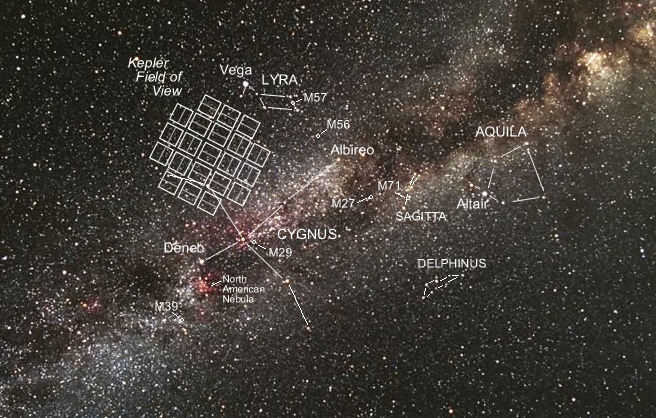
\includegraphics[width=0.95\textwidth]{figures/kepler_fov.png}
	\end{center}
\end{frame}

\begin{frame}{Neurális hálók}
    \begin{itemize}
        \item Neurális hálókkal osztályozás példa: \href{https://www.tensorflow.org/tutorials/keras/classification}{Ruhák (TensorFlow)}
    \end{itemize}
    
    \centering
    \begin{tikzpicture}
            \node (-2,0) (cipo) {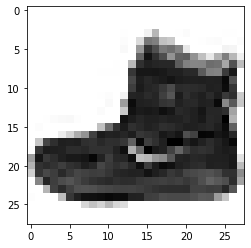
\includegraphics[width=0.2\textwidth]{figures/boot.png}};
            \draw (3,-1) rectangle (5,1);
            \draw (4,0) node {\small{Neurális háló}};
            \draw [->] (1.2, 0) -- (2.9,0);
            \draw [->] (5.1, 0) -- (6,0);
            \draw (6.4,0) node {Cipő};
    \end{tikzpicture}
    
    \pause
    \centering
    \begin{tikzpicture}
            \node (-2,0) (cipo) {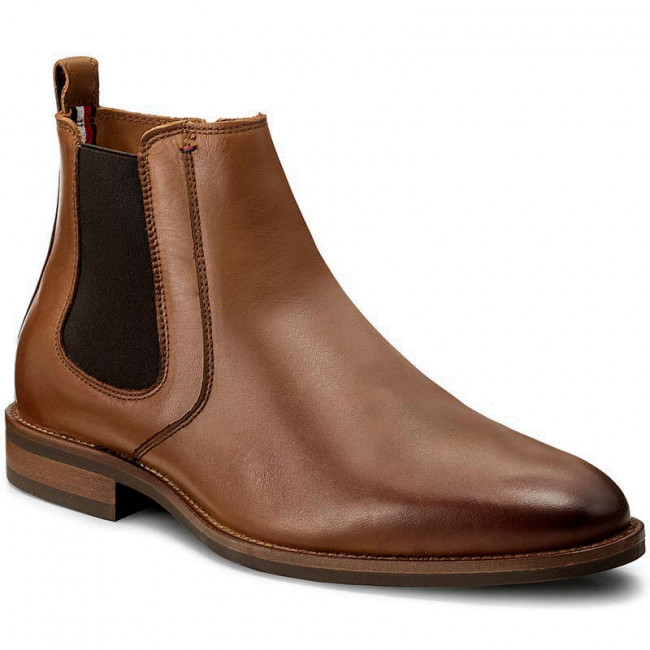
\includegraphics[width=0.2\textwidth]{figures/boot2.jpg}};
            \draw (3,-1) rectangle (5,1);
            \draw (4,0) node {\small{Neurális háló}};
            \draw [->] (1.2, 0) -- (2.9,0);
            \draw [->] (5.1, 0) -- (6,0);
            \draw (6.4,0) node {???};
    \end{tikzpicture}
\end{frame}

\begin{frame}{Konvolúciós neurális hálók}
    \begin{itemize}
        \item Ötlet 1: szűrjünk a képen, mielőtt tanítunk
    \end{itemize}
    
    \centering
    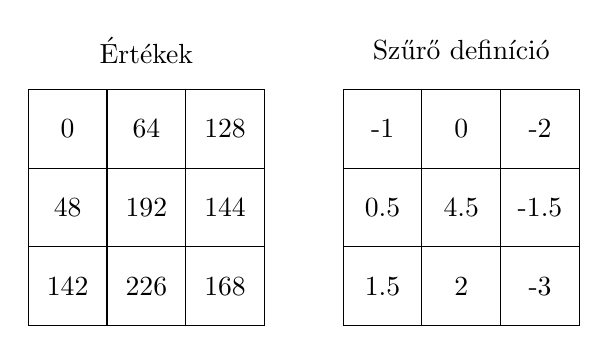
\begin{tikzpicture}
        \foreach \x in {1,2,3,5,6,7} {
            \foreach \y in {1,2,3} {
                \draw (\x,\y) +(-.5, -.5) rectangle ++(.5,.5);
                % \draw (\x,\y) node {\x,\y};
            }
        }
        \draw (1,1) node {142}
              (2,1) node {226}
              (3,1) node {168}
              (1,2) node {48}
              (2,2) node {192}
              (3,2) node {144}
              (1,3) node {0}
              (2,3) node {64}
              (3,3) node {128};
              
        \draw (5,1) node {1.5}
              (6,1) node {2}
              (7,1) node {-3}
              (5,2) node {0.5}
              (6,2) node {4.5}
              (7,2) node {-1.5}
              (5,3) node {-1}
              (6,3) node {0}
              (7,3) node {-2};
        
        \draw (2,4) node {Értékek}
              (6,4) node {Szűrő definíció};
    \end{tikzpicture}
    
    \vspace*{0.5cm}
    192 új értéke:\\
    $(-1*0) + (0*64) + (-2*128) + (0.5 * 48) + (4.5 * 192) + (-1.5 * 144) + (1.5 * 42) + (2 * 226) + (-3 * 168)$
\end{frame}

\begin{frame}{Konvolúciós neurális hálók}
    \centering
    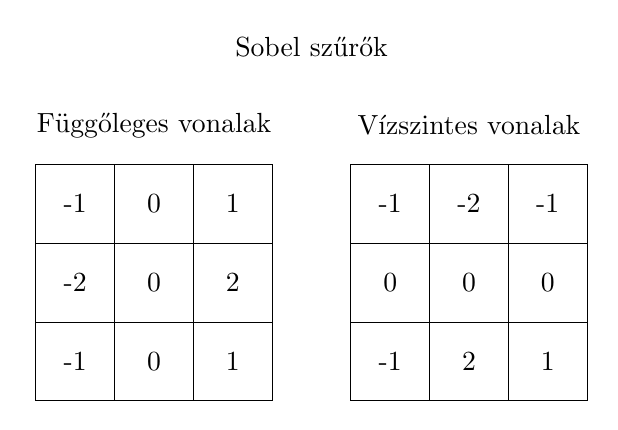
\begin{tikzpicture}
        \foreach \x in {1,2,3,5,6,7} {
            \foreach \y in {1,2,3} {
                \draw (\x,\y) +(-.5,-.5) rectangle ++(.5,.5);
            }
        }
        
        \draw (1,1) node {-1}
              (2,1) node {0}
              (3,1) node {1}
              (1,2) node {-2}
              (2,2) node {0}
              (3,2) node {2}
              (1,3) node {-1}
              (2,3) node {0}
              (3,3) node {1};
              
        \draw (5,1) node {-1}
              (6,1) node {2}
              (7,1) node {1}
              (5,2) node {0}
              (6,2) node {0}
              (7,2) node {0}
              (5,3) node {-1}
              (6,3) node {-2}
              (7,3) node {-1};
              
        \draw (4,5) node {Sobel szűrők}
              (2,4) node {Függőleges vonalak}
              (6,4) node {Vízszintes vonalak};
    \end{tikzpicture}
\end{frame}

\begin{frame}{Konvolúciós neurális hálók}
    \begin{itemize}
        \item Ötlet 2: Pooling: pixeleket csoportosít és tovább szűr
    \end{itemize}
    
    \centering
    \begin{tikzpicture}[scale=0.6]
        \draw (2,6.5) node {Maxpooling 2x2:};
    
        \path [draw=lorange,fill=lorange!80,thick] (0.5,2.5) rectangle (2.5,4.5);
        \path [draw=lorange,fill=lorange!80,thick] (5.5,5.5) rectangle (7.5,7.5);
        \path [draw=lorange,fill=lorange!80,thick] (9.5,6) rectangle (10.5,7);
        \path [draw=lorange,fill=lorange!80,thick] (14.5,1.5) rectangle (15.5,2.5);
        
        \path [draw=lblue,fill=lblue!80,thick] (2.5,2.5) rectangle (4.5,4.5);
        \path [draw=lblue,fill=lblue!80,thick] (5.5,2.5) rectangle (7.5,4.5);
        \path [draw=lblue,fill=lblue!80,thick] (9.5,3) rectangle (10.5,4);
        \path [draw=lblue,fill=lblue!80,thick] (15.5,1.5) rectangle (16.5,2.5);

        \path [draw=dblue,fill=dblue!80,thick] (0.5,0.5) rectangle (2.5,2.5);
        \path [draw=dblue,fill=dblue!80,thick] (5.5,-0.5) rectangle (7.5,1.5);
        \path [draw=dblue,fill=dblue!80,thick] (9.5,0) rectangle (10.5,1);
        \path [draw=dblue,fill=dblue!80,thick] (14.5,0.5) rectangle (15.5,1.5);
        
        \path [draw=dorange,fill=dorange!80,thick] (2.5,0.5) rectangle (4.5,2.5);
        \path [draw=dorange,fill=dorange!80,thick] (5.5,-3.5) rectangle (7.5,-1.5);
        \path [draw=dorange,fill=dorange!80,thick] (9.5,-3) rectangle (10.5,-2);
        \path [draw=dorange,fill=dorange!80,thick] (15.5,0.5) rectangle (16.5,1.5);
    
        \foreach \x in {1,2,3,4} {
            \foreach \y in {1,2,3,4} {
                \draw (\x,\y) +(-.5,-.5) rectangle ++(.5,.5);
            }
        }
        
        \foreach \x in {6,7} {
            \foreach \y in {-3,-2,0,1,3,4,6,7} {
                \draw (\x,\y) +(-.5,-.5) rectangle ++(.5,.5);
            }
        }
        
        \foreach \y in {-2.5,0.5,3.5,6.5} {
            \draw (10,\y) +(-.5,-.5) rectangle ++(.5,.5);
        }
        
        \foreach \x in {15,16} {
            \foreach \y in {1,2} {
                \draw (\x,\y) +(-.5,-.5) rectangle ++(.5,.5);
            }
        }
        
        \draw (1,1) node {\footnotesize 255}
              (2,1) node {\footnotesize 0}
              (3,1) node {\footnotesize 0}
              (4,1) node {\footnotesize 64}
              (1,2) node {\footnotesize 142}
              (2,2) node {\footnotesize 226}
              (3,2) node {\footnotesize 168}
              (4,2) node {\footnotesize 0}
              (1,3) node {\footnotesize 48}
              (2,3) node {\footnotesize 192}
              (3,3) node {\footnotesize 144}
              (4,3) node {\footnotesize 144}
              (1,4) node {\footnotesize 0}
              (2,4) node {\footnotesize 64}
              (3,4) node {\footnotesize 128}
              (4,4) node {\footnotesize 128};
              
        \draw (6,-3) node {\footnotesize 0}
              (7,-3) node {\footnotesize 64}
              (6,-2) node {\footnotesize 168}
              (7,-2) node {\footnotesize 0}
              (6,0) node {\footnotesize 255}
              (7,0) node {\footnotesize 0}
              (6,1) node {\footnotesize 142}
              (7,1) node {\footnotesize 226}
              (6,3) node {\footnotesize 144}
              (7,3) node {\footnotesize 144}
              (6,4) node {\footnotesize 128}
              (7,4) node {\footnotesize 128}
              (6,6) node {\footnotesize 48}
              (7,6) node {\footnotesize 192}
              (6,7) node {\footnotesize 0}
              (7,7) node {\footnotesize 64};
              
        \draw (10,-2.5) node {\footnotesize 168}
              (10,0.5) node {\footnotesize 255}
              (10,3.5) node {\footnotesize 144}
              (10,6.5) node {\footnotesize 192};
              
        \draw (15,1) node {\footnotesize 255}
              (16,1) node {\footnotesize 168}
              (15,2) node {\footnotesize 192}
              (16,2) node {\footnotesize 144};
        
        % \draw [->] (1.5,4.5) -- (5.5,6.5);
        \foreach \y in {-2.5,0.5,3.5,6.5} {
            \draw [->] (7.5,\y) -- (9.5,\y);
        }
        
        \draw [->] (10.5,6.5) -- (14.5,2);
        \draw [->] (10.5,3.5) -- (16,2.5);
        \draw [->] (10.5,0.5) -- (14.5,1);
        \draw [->] (10.5,-2.5) -- (16,0.5);
    \end{tikzpicture}
\end{frame}

\begin{frame}{Konvolúciós neurális hálók}
    \begin{itemize}
        \item \href{https://www.cs.ryerson.ca/~aharley/vis/conv/}{Számfelismerő}
        \item \href{https://poloclub.github.io/cnn-explainer/}{Konvolúciós neurális hálók interaktív vizualizálása}
    \end{itemize}
\end{frame}

\begin{frame}{A Kepler-80 g és Kepler-90 i esete}
    \centering
    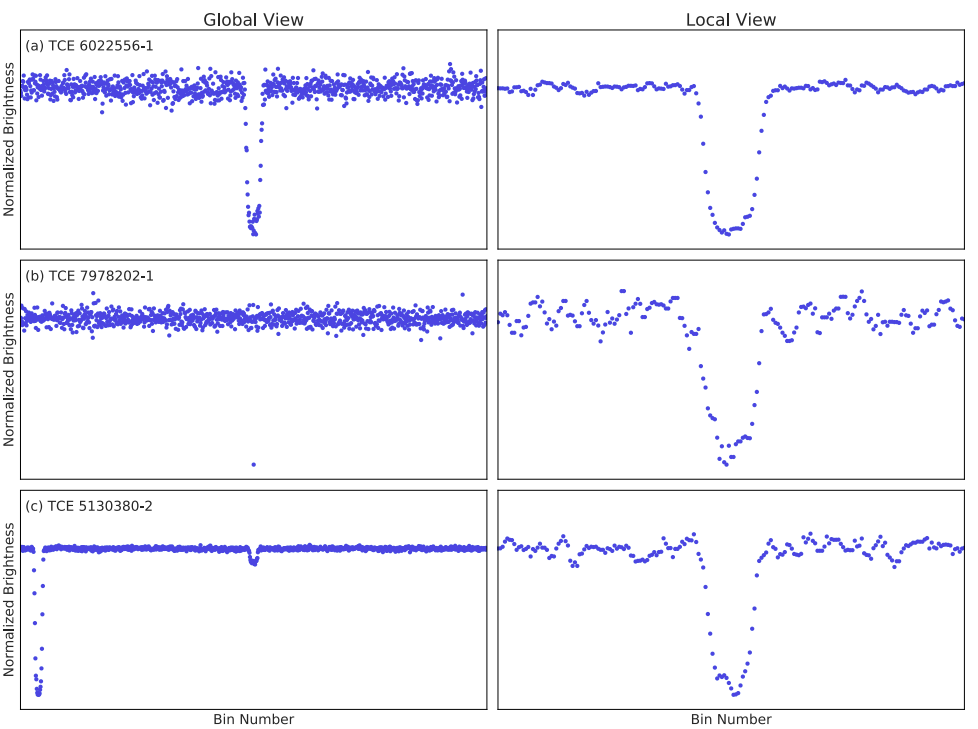
\includegraphics[width=0.8\textwidth]{figures/kepler_tce_views.png}
\end{frame}

\begin{frame}{A Kepler-80 g és Kepler-90 i esete}
    \centering
    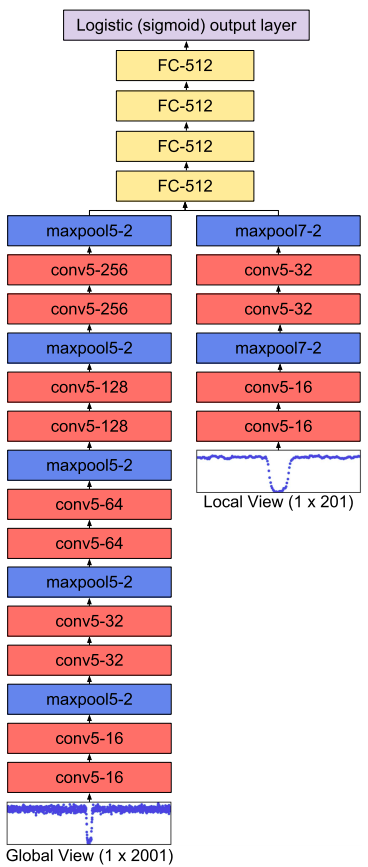
\includegraphics[height=0.85\textheight]{figures/kepler-80-cnn.png}
\end{frame}

\begin{frame}{A Kepler-80 g és Kepler-90 i esete}
    \centering
    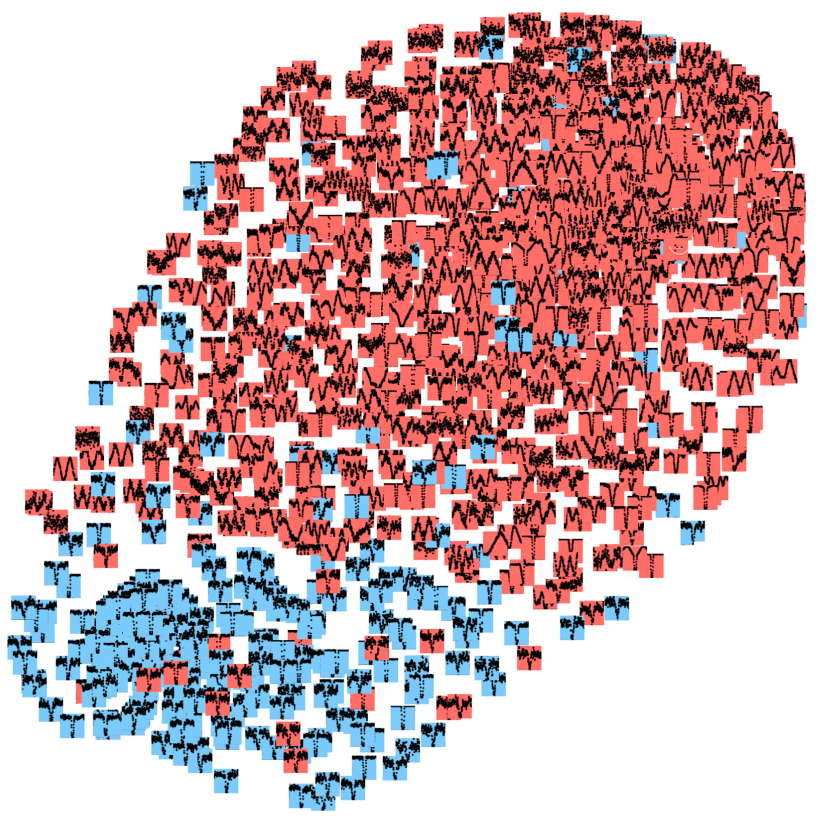
\includegraphics[width=0.6\textwidth]{figures/kepler80-tsne.png}
\end{frame}

\begin{frame}{A Kepler-80 g és Kepler-90 i esete}
    \begin{itemize}
        \item 670 többes rendszer jelölt
        \item 157 jelölt eldobása: 30 percnél rövidebb fedés, nincs három fedés a teljes fénygörbében
        \item 513 marad
        \item ebből 30-nak 50\%-nál nagyobb az esélye, hogy bolygó
        \item 9-nek 80\%-nál nagyobb az esélye
        \item 4-nek 90\%-nál nagyobb az esélye
        \item 1 spektroszkópiai kettős
        \item 1-nél műszeres effektusok zavarnak
        \item 2 bolygó
    \end{itemize}
\end{frame}

\begin{frame}{A Kepler-80 g és Kepler-90 i esete}
    \centering
    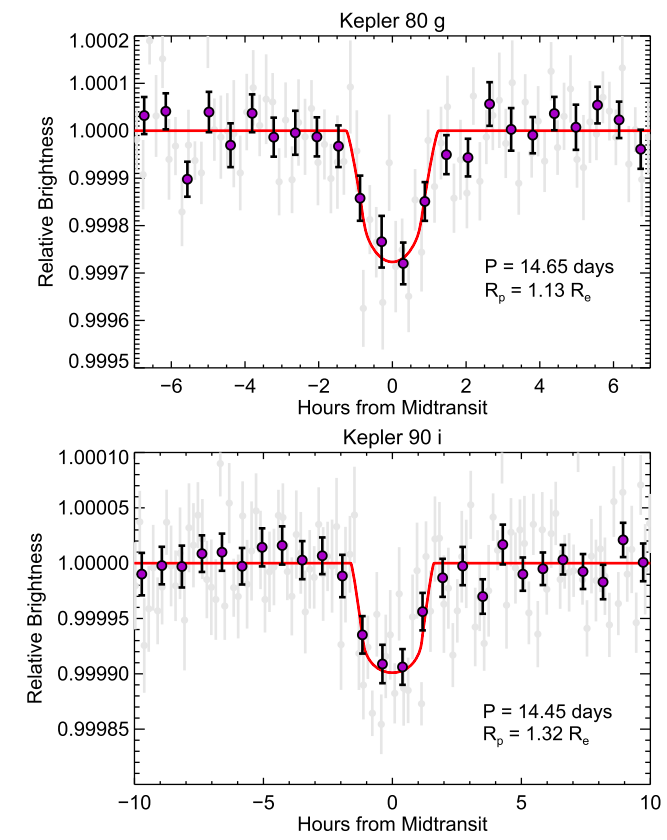
\includegraphics[width=0.5\textwidth]{figures/kepler-80-90-transit.png}
\end{frame}
